\documentclass[11pt, fleqn]{article}

\usepackage{amsmath}
\usepackage{amssymb}
\usepackage{amsthm}
\usepackage{mathtools}
\usepackage{hyperref}
\usepackage{ulem}
\usepackage{enumitem}
\usepackage[left=0.75in, right=0.75in, bottom=0.75in, top=1.0in]{geometry}
\usepackage{floatrow}
\usepackage{graphicx}
\usepackage[export]{adjustbox}

\usepackage{sectsty}
\sectionfont{\centering}

\usepackage[perpage]{footmisc}

\usepackage{fancyhdr}
\pagestyle{fancy}
\fancyhf{}
\lhead{190100036 \& 190100044 \& 190100055}
\rhead{CS 252: Lab 1}
\renewcommand{\footrulewidth}{1.0pt}
\cfoot{Page \thepage}

\setlength{\parindent}{0em}
\renewcommand{\arraystretch}{2}%

\title{CS 252: Lab 1}
\author{
\begin{tabular}{|c|c|c|}
     \hline
     Krushnakant Bhattad & Devansh Jain & Harshit Varma \\
     \hline
     190100036 & 190100044 & 190100055 \\
     \hline
\end{tabular}
}
% \author{
%   Krushnakant Bhattad\\
%   190100036
%   \and
%   Devansh Jain\\
%   190100044
%   \and
%   Harshit Varma\\
%   190100055
% }
\date{\today}

\usepackage{hyperref}

\usepackage[dvipsnames]{xcolor}

\begin{document}

\maketitle
\tableofcontents
\thispagestyle{empty}
\setcounter{page}{0}
\renewcommand{\arraystretch}{1}

\newpage 
\section*{Part (a)}
\label{parta}
\addcontentsline{toc}{section}{Part (a)}
\setcounter{equation}{0}
\setcounter{figure}{0}

\textit{Record signal strength over some geographical area,
and pictorially represent it on a map. Use colours to say if the signal strength is good or bad etc. State the range of signal strengths (in dBm) which correspond to different colours. (15 marks)}

\begin{figure}[H]
    \centering
    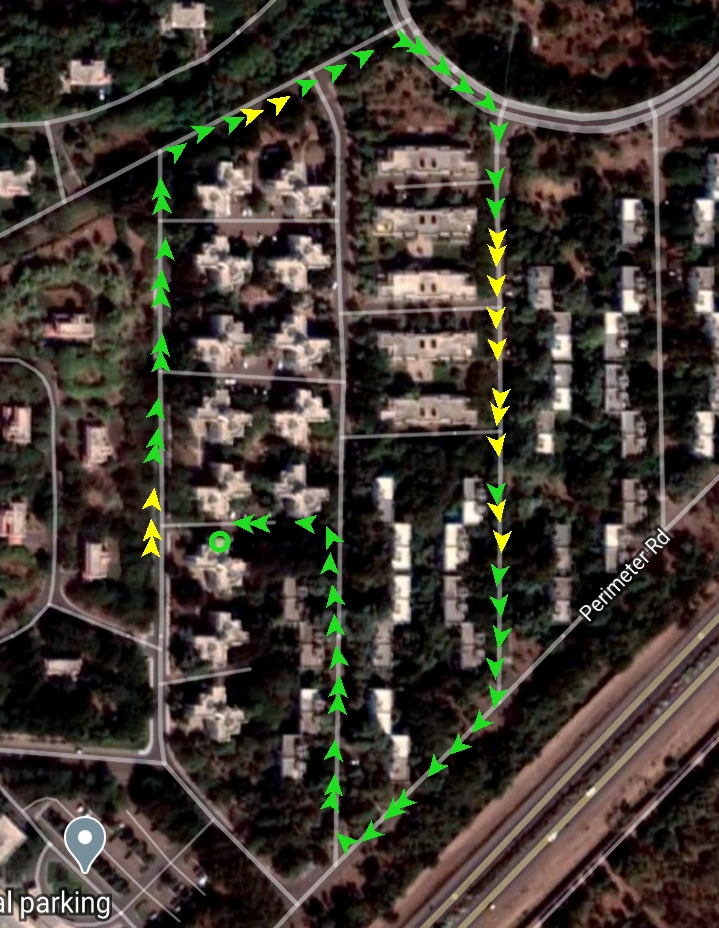
\includegraphics[scale = 0.5, angle = 90]{path_map.jpg}
    \caption{Area over which the signal strength was recorded}
    \label{fig:my_label}
\end{figure}

\subsection*{Color Scheme:} 
In the above map, the parts of the path covered by \textcolor{ForestGreen}{green} arrows
indicate a good signal strength; 
while those covered by \textcolor{Apricot}{yellow} indicate 
a relatively bad signal strength.\\

The signals received varied from \textbf{-92} dBm\footnote{dBm:  decibels per milliwatt} to \textbf{-52} dBm, with a mean of \textbf{-74.11} dBm and a standard deviation of \textbf{9.66} dBm

\subsection*{Ranges covered by different colours:}

\textcolor{ForestGreen}{green} covers the range \textbf{-50 dBm} to \textbf{-85 dBm}\\
\textcolor{Apricot}{yellow} covers the range \textbf{-85 dBm} to \textbf{-105 dBm}


\newpage
\section*{Part (b)}
\addcontentsline{toc}{section}{Part (b)}
\setcounter{equation}{0}
\setcounter{figure}{0}

\textit{Make a list of all the unique base-stations (\texttt{eNodeBIDs}) your phone was connected to, during the measurement. (5 marks)}

\medskip

The set of eNBIDs that the phone connected to are: 
$\mathbf{\{ 5318, 5482, 6378, 12987, 13532 \}}$\\
(Attach the annotated base stations screenshot here)

\newpage
\section*{Part (c)}
\addcontentsline{toc}{section}{Part (c)}
\setcounter{equation}{0}
\setcounter{figure}{0}

\textit{State in words in your report what you think the reasons for poor signal strength were. If you can annotate your map to show obstacles etc, that would be even better, but this is not essential. (5 marks)}


\newpage
\section*{Part (d)}
\addcontentsline{toc}{section}{Part (d)}
\setcounter{equation}{0}
\setcounter{figure}{0}

\textit{Comment if when you are standing in a fixed location (when you are not moving) if the signal strength (RSRP: reference signal received power) is steady or if it varies, based on a measurement of a minute’s duration. Give a plot of how RSRP varies with time at a fixed location. (5 marks)}

\begin{figure}[H]
    \centering
    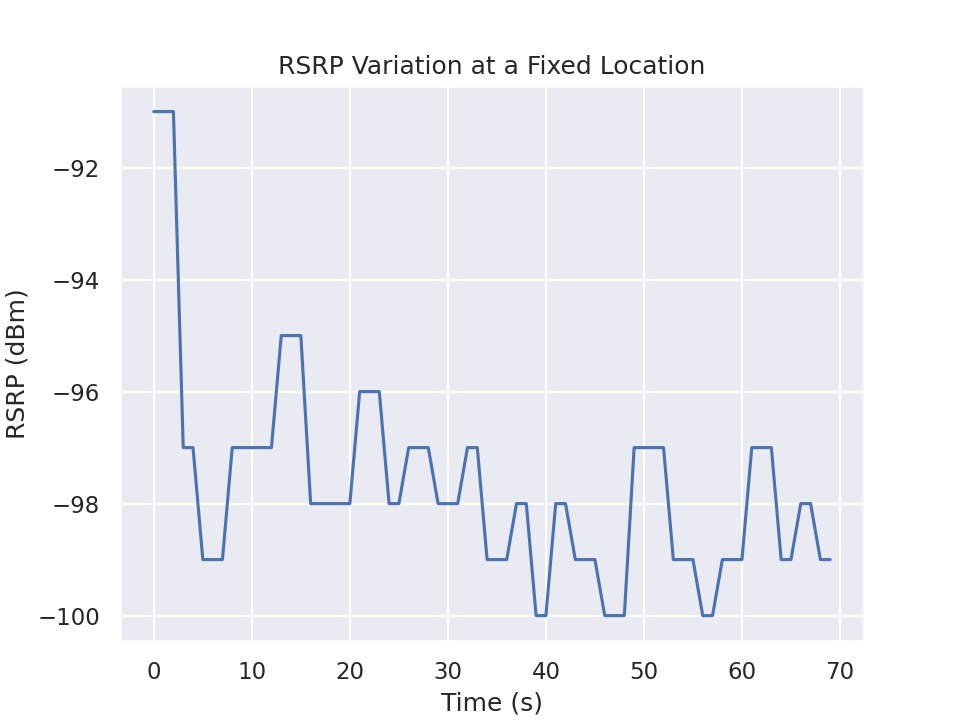
\includegraphics[scale = 1]{part_d.jpg}
    \caption{RSRP Variation at a Fixed Location}
\end{figure}

While standing at a fixed location 
\footnote{Measurements were taken in a confined space} 
for about 70 seconds, the signal strength varies between \textbf{-100} and
\textbf{-91} dBm, having a mean value of \textbf{-97.69} dBm and a standard deviation of \textbf{1.89} dBm\\

This is still much less than the variation seen in \nameref{parta}, which varied from -92 dBm to -52 dBm, with a mean of -74.11 dBm and a standard deviation of 9.66 dBm\\

We believe that this small variation, seen at a fixed location can be attributed to:
\begin{enumerate}[itemsep=-1ex]
    \item Local interference from neighbouring devices
    \item Natural noise while data acquisition 
\end{enumerate}


\newpage
\section*{Appendix}
\addcontentsline{toc}{section}{Appendix}
\setcounter{equation}{0}
\setcounter{figure}{0}

\subsection*{Screenshots}


\end{document}